\documentclass[aspectratio=169,10pt]{beamer}
% =====================================================================
%  Le Collé — thème de présentation (même palette et mêmes notations que la fiche)
% =====================================================================
\usepackage[utf8]{inputenc}
\usepackage[T1]{fontenc}
\usepackage[sc]{mathpazo}
\usepackage[scaled=0.92]{helvet}
\usefonttheme{professionalfonts}
\usepackage{amsmath,amssymb,mathrsfs,stmaryrd}
\usepackage{microtype}
\usepackage{booktabs,array,multicol}
\usepackage[most]{tcolorbox}
\usepackage{tikz,pgfplots}
\usetikzlibrary{arrows.meta,calc,positioning,decorations.pathreplacing,shapes.misc}
\pgfplotsset{compat=1.17,trig format plots=rad}
\usepackage{tkz-tab}

% ---------- palette (identique à la fiche) ----------
\definecolor{Ink}{HTML}{1C2533}\definecolor{Bleu}{HTML}{1F3A5F}\definecolor{BleuMoyen}{HTML}{4A6A8F}
\definecolor{BleuClair}{HTML}{9DB2C9}\definecolor{Fond}{HTML}{F2F4F7}\definecolor{Ocre}{HTML}{B07A26}
\definecolor{Brique}{HTML}{A23B2A}\definecolor{Gris}{HTML}{5E6672}\definecolor{Filet}{HTML}{C5CCD6}
\definecolor{Vert}{HTML}{2E6B4F}

% ---------- notations (identiques à la fiche) ----------
\newcommand{\K}{\mathbb{K}}\newcommand{\R}{\mathbb{R}}\newcommand{\C}{\mathbb{C}}\newcommand{\Z}{\mathbb{Z}}
\newcommand{\Mn}[1]{\mathcal{M}_{n}(#1)}\newcommand{\rg}{\operatorname{rg}}\newcommand{\vect}{\operatorname{Vect}}
\newcommand{\Mat}{\operatorname{Mat}}\newcommand{\Id}{\operatorname{Id}}\newcommand{\com}{\operatorname{com}}
\newcommand{\vv}[1]{\overrightarrow{#1}}\newcommand{\ve}[1]{\vec{#1}}
\newcommand{\dt}[1]{\left|\begin{matrix}#1\end{matrix}\right|}
\DeclareRobustCommand{\HP}{{\sffamily\bfseries\scriptsize\textcolor{Brique}{[HP]}}}

% ---------- réglages beamer ----------
\setbeamertemplate{navigation symbols}{}
\setbeamersize{text margin left=0.85cm,text margin right=0.85cm}
\setbeamercolor{normal text}{fg=Ink,bg=white}
\setbeamercolor{structure}{fg=Bleu}
\setbeamercolor{alerted text}{fg=Brique}
\setbeamerfont{alerted text}{series=\bfseries}
\setbeamertemplate{itemize item}{\raisebox{0.15em}{\textcolor{Ocre}{\rule{0.38em}{0.38em}}}}
\setbeamertemplate{itemize subitem}{\textcolor{BleuMoyen}{\scriptsize\textbullet}}
\setbeamertemplate{enumerate item}{\textcolor{Bleu}{\sffamily\bfseries\insertenumlabel.}}
\setlength{\leftmargini}{1.2em}
\setbeamertemplate{blocks}[default]

% numéro de la partie courante, rappelé dans le titre et le pied de page (renvoi à la fiche)
\def\fichesec{}\def\chapnom{}
\newcommand{\chapitre}[1]{\def\chapnom{#1}}

\setbeamertemplate{frametitle}{%
  \vskip0.28cm
  \ifx\fichesec\empty\else
    \tikz[baseline=(b.base)]\node[fill=Ocre,text=white,font=\sffamily\bfseries\scriptsize,inner sep=2.5pt,rounded corners=1pt](b){\fichesec};\hspace{0.45em}%
  \fi
  {\color{Bleu}\sffamily\bfseries\Large\insertframetitle}\par
  \vskip0.06cm{\color{Filet}\rule{\linewidth}{0.5pt}}\vskip-0.2cm}

\setbeamertemplate{footline}{%
  \hbox to\paperwidth{%
    \hspace*{0.85cm}{\scriptsize\sffamily\color{Gris}Le Collé\ \ \textcolor{Filet}{|}\ \ \chapnom}\hfill
    {\scriptsize\sffamily\color{Gris}\ifx\fichesec\empty\else fiche \textbf{\color{Ocre}§\fichesec}\quad\fi\insertframenumber}\hspace*{0.85cm}}%
  \vskip0.18cm
  \hbox{\begin{tikzpicture}
    \fill[Fond] (0,0) rectangle (\paperwidth,2.2pt);
    \pgfmathsetmacro\prog{min(\insertframenumber/max(\inserttotalframenumber,1),1)}
    \fill[Ocre] (0,0) rectangle ({\prog*\paperwidth},2.2pt);
  \end{tikzpicture}}}

% ---------- encadrés : même code couleur que la fiche ----------
\tcbset{sb/.style={enhanced,arc=1pt,boxrule=0pt,left=6pt,right=6pt,top=3pt,bottom=3pt,before skip=0.14cm,after skip=0.14cm,
  fontupper=\normalsize\raggedright}}
\newcommand{\etiq}[2]{{\sffamily\bfseries\scriptsize\color{#1}\MakeUppercase{#2}}\par\vspace{2pt}}
\newtcolorbox{DEF}[1][Définition]{sb,colback=white,borderline west={2pt}{0pt}{Bleu},before upper={\etiq{Bleu}{#1}}}
\newtcolorbox{PROP}[1][Propriété]{sb,colback=Fond,borderline west={3pt}{0pt}{Bleu},before upper={\etiq{Bleu}{#1}}}
\newtcolorbox{FORM}[1][Formule]{sb,colback=white,colframe=BleuMoyen,boxrule=0.6pt,before upper={\etiq{BleuMoyen}{#1}}}
\newtcolorbox{METH}[1]{sb,colback=white,borderline north={1pt}{0pt}{Bleu},borderline south={1pt}{0pt}{Bleu},
  before upper={{\sffamily\bfseries\scriptsize\colorbox{Bleu}{\color{white}MÉTHODE}\ \color{Bleu}#1}\par\vspace{3pt}}}
\newtcolorbox{PIEGE}[1][Piège]{sb,colback=Brique!6,borderline west={2pt}{0pt}{Brique},before upper={\etiq{Brique}{#1}}}
\newtcolorbox{ASTU}[1][Astuce]{sb,colback=Ocre!8,borderline west={2pt}{0pt}{Ocre},before upper={\etiq{Ocre}{#1}}}
\newtcolorbox{HPBOX}{sb,colback=white,borderline west={2pt}{0pt}{Brique},before upper={\etiq{Brique}{Hors programme}}}
\newtcolorbox{ATOI}[1][À toi]{sb,colback=Vert!6,borderline west={2pt}{0pt}{Vert},before upper={\etiq{Vert}{#1}}}
\newtcolorbox{RETENIR}{sb,colback=Bleu!5,colframe=Bleu,boxrule=0.8pt,left=8pt,
  before upper={\etiq{Bleu}{À retenir}}}
\newtcolorbox{EX}[1][Exemple]{sb,colback=white,colframe=Filet,boxrule=0.5pt,before upper={\etiq{Gris}{#1}}}

% complément pédagogique absent du livre : étiquette pointillée
\DeclareRobustCommand{\ajout}{\tikz[baseline=(a.base)]\node[draw=Gris,dashed,text=Gris,font=\sffamily\scriptsize,inner sep=2pt,rounded corners=1pt](a){complément hors livre};}
\DeclareRobustCommand{\livre}[1]{{\sffamily\scriptsize\color{Gris}[livre #1]}}
\newcommand{\rep}[1]{\textcolor{Vert}{#1}}% réponse attendue de l'élève

% ---------- styles de figures (identiques au livre) ----------
\pgfplotsset{courbe/.style={axis lines=middle,axis equal image,
  axis line style={Gris,-{Stealth[length=4pt]}},
  xlabel={$x$},ylabel={$y$},ticklabel style={font=\scriptsize\sffamily,color=Gris},
  every axis x label/.style={at={(ticklabel* cs:1)},anchor=west,font=\small},
  every axis y label/.style={at={(ticklabel* cs:1)},anchor=south,font=\small},
  samples=200,smooth}}
\pgfplotsset{mini/.style={axis lines=middle,axis line style={Filet},xtick=\empty,ytick=\empty,width=3.9cm,height=3.9cm,
  xmin=-1.15,xmax=1.15,ymin=-1.15,ymax=1.15,title style={font=\footnotesize\sffamily,yshift=-0.1cm},samples=100}}
\tikzset{arcetude/.style={Bleu,line width=1.25pt},
         reste/.style={BleuClair,line width=1pt},
         tgte/.style={Ocre,line width=1pt},
         asy/.style={Gris,dashed,line width=0.7pt},
         pt/.style={circle,fill=Ink,inner sep=1.3pt},
         >={Stealth[length=5pt]}}

% ---------- diapositives de partie ----------
% \partie{num}{titre}{question guide}{liste des parties du chapitre via \rm}
\newcommand{\rmitem}[2]{\def\tmp{#1}%
  \ifx\tmp\fichesec{\color{Bleu}\bfseries #1\quad #2}\else{\color{Gris!70}#1\quad #2}\fi\par\vspace{2pt}}
\newcommand{\partie}[4]{%
  \def\fichesec{#1}\section{#2}%
  \begin{frame}[plain]
  \begin{tikzpicture}[remember picture,overlay]
    \fill[Bleu] (current page.north west) rectangle ([xshift=6.3cm]current page.south west);
    \node[anchor=north west,text=white,font=\sffamily\bfseries\fontsize{40}{40}\selectfont] at ([xshift=0.8cm,yshift=-1.2cm]current page.north west) {#1};
    \node[anchor=north west,text width=4.8cm,align=left,text=white,font=\sffamily\bfseries\Large] at ([xshift=0.8cm,yshift=-2.9cm]current page.north west) {\hyphenpenalty=10000\exhyphenpenalty=10000 #2\par};
    \node[anchor=south west,text width=4.8cm,text=white!75!Bleu,font=\sffamily\scriptsize] at ([xshift=0.8cm,yshift=0.6cm]current page.south west) {\chapnom\\fiche \textbf{§#1}};
  \end{tikzpicture}
  \hspace*{5.5cm}\begin{minipage}{8.4cm}
  {\sffamily\scriptsize\color{Ocre}\bfseries LA QUESTION}\par\vspace{2pt}
  {\large #3}\par\vspace{0.7cm}
  {\sffamily\scriptsize\color{Gris}\bfseries DANS CE CHAPITRE}\par\vspace{4pt}
  {\sffamily\small #4}
  \end{minipage}
  \end{frame}}



% ---------- exercices en séance : énoncé sur une diapositive, correction sur la suivante ----------
\newcommand{\badgeexo}[1]{\tikz[baseline=(e.base)]\node[fill=Vert,text=white,font=\sffamily\bfseries\scriptsize,inner sep=2.5pt,rounded corners=1pt](e){EXERCICE #1};\hspace{0.4em}}
\newcommand{\badgecor}[1]{\tikz[baseline=(e.base)]\node[draw=Vert,line width=0.8pt,text=Vert,font=\sffamily\bfseries\scriptsize,inner sep=2.2pt,rounded corners=1pt](e){CORRECTION #1};\hspace{0.4em}}
\newtcolorbox{ENONCE}[1][]{sb,colback=Vert!6,borderline west={3pt}{0pt}{Vert},left=9pt,top=5pt,bottom=5pt,
  before upper={{\sffamily\bfseries\scriptsize\color{Vert}À TOI\ifx\relax#1\relax\else\ \ ·\ \ \MakeUppercase{#1}\fi}\par\vspace{4pt}}}
\newtcolorbox{INDICE}{sb,colback=white,colframe=Vert!60,boxrule=0.5pt,borderline={0.5pt}{0pt}{Vert!60,dashed},
  before upper={\etiq{Vert}{Indice (si besoin)}}}
\newtcolorbox{RAIS}[1][Le raisonnement]{sb,colback=Vert!5,borderline west={2pt}{0pt}{Vert},before upper={\etiq{Vert}{#1}}}
\newtcolorbox{OUTIL}{sb,colback=Fond,borderline west={2pt}{0pt}{Bleu},before upper={\etiq{Bleu}{Propriété ou méthode utilisée}}}
\newcommand{\etape}[1]{{\sffamily\bfseries\footnotesize\color{Vert}#1}\ }
\newcommand{\objectif}[1]{\par\vspace{2pt}{\footnotesize\sffamily\color{Gris}Objectif : #1}}
\newcommand{\Ker}{\operatorname{Ker}}\renewcommand{\Im}{\operatorname{Im}}\newcommand{\tr}{\operatorname{tr}}\newcommand{\Sp}{\operatorname{Sp}}
\newcommand{\GLn}[1]{\mathrm{GL}_n(#1)}
\title{Le Collé --- Algèbre linéaire et réduction}

\begin{document}

% ---------------------------------------------------------------- titre
\begin{frame}[plain]
\begin{tikzpicture}[remember picture,overlay]
  \fill[Bleu] (current page.north west) rectangle (current page.south east);
  \node[anchor=north west,text=white!70!Bleu,font=\sffamily\scriptsize] at ([xshift=1cm,yshift=-1.2cm]current page.north west)
    {LE COLLÉ\ \ ·\ \ MATHÉMATIQUES PT\ \ ·\ \ CHAPITRE 2\ \ ·\ \ SUPPORT DE SÉANCE};
  \node[anchor=north west,text=white,font=\sffamily\bfseries\fontsize{26}{30}\selectfont,text width=13cm] at ([xshift=1cm,yshift=-2.1cm]current page.north west)
    {Algèbre linéaire\\ et réduction};
  \fill[Ocre] ([xshift=1cm,yshift=-4.6cm]current page.north west) rectangle ([xshift=4cm,yshift=-4.65cm]current page.north west);
  \node[anchor=north west,text=white!80!Bleu,font=\normalsize,text width=12.5cm] at ([xshift=1cm,yshift=-5cm]current page.north west)
    {Présentation pour expliquer, avec neuf exercices à chercher en séance ;\\ le \textbf{livre} pour relire, la \textbf{fiche} pour réviser.
     Mêmes parties (§1.1 à §1.8), mêmes notations.};
\end{tikzpicture}
\end{frame}

% ---------------------------------------------------------------- mode d'emploi
\begin{frame}{Comment utiliser ce support}
\vspace{-0.15cm}
\begin{columns}[T]
\column{0.48\textwidth}
\begin{DEF}vocabulaire à connaître\end{DEF}\vspace{-9pt}
\begin{PROP}[Propriété / théorème]énoncé précis, avec ses hypothèses\end{PROP}\vspace{-9pt}
\begin{METH}{}démarche à suivre, étape par étape\end{METH}\vspace{-9pt}
\begin{PIEGE}erreur classique à éviter\end{PIEGE}
\column{0.48\textwidth}
\begin{ENONCE}[durée indicative]exercice à chercher en séance : diapositive \textbf{seule}, la correction est sur la suivante\end{ENONCE}\vspace{-9pt}
\begin{RAIS}correction : d'abord le raisonnement, puis la méthode, puis les étapes\end{RAIS}\vspace{-9pt}
\begin{ASTU}technique qui fait gagner du temps\end{ASTU}\vspace{-9pt}
\begin{RETENIR}l'essentiel d'une partie\end{RETENIR}
\end{columns}
{\footnotesize Les badges \badgeexo{1} et \badgecor{1} repèrent les exercices et leurs corrections. Le numéro ocre
\tikz[baseline=(b.base)]\node[fill=Ocre,text=white,font=\sffamily\bfseries\scriptsize,inner sep=2pt](b){1.2}; renvoie à la partie de la fiche.}
\end{frame}

% ---------------------------------------------------------------- plan
\begin{frame}{Plan : deux séances de 2 h}
\begin{columns}[T]
\column{0.56\textwidth}
\small
\renewcommand{\arraystretch}{1.3}
\begin{tabular}{@{}l l r@{}}
\multicolumn{3}{@{}l}{\sffamily\bfseries\color{Ocre}Séance 1 --- le langage}\\
\textbf{\color{Bleu}1.1} & Semblables, sommes directes, trace & \color{Vert}Ex.~1, 2\\
\textbf{\color{Bleu}1.2} & Sous-espaces stables & \color{Vert}Ex.~3\\
\textbf{\color{Bleu}1.3} & Éléments propres & \color{Vert}Ex.~4\\
\textbf{\color{Bleu}1.4} & Polynôme caractéristique & \color{Vert}Ex.~5\\[2pt]
\multicolumn{3}{@{}l}{\sffamily\bfseries\color{Ocre}Séance 2 --- la réduction}\\
\textbf{\color{Bleu}1.5} & Diagonalisation & \color{Vert}Ex.~6, 7\\
\textbf{\color{Bleu}1.6} & Applications & \color{Vert}Ex.~8\\
\textbf{\color{Bleu}1.7} & Trigonalisation & \color{Vert}Ex.~9\\
\textbf{\color{Bleu}1.8} & Synthèse &
\end{tabular}
\column{0.4\textwidth}
\begin{ASTU}[Le fil du chapitre]
\small Une seule question : \textbf{dans quelle base la matrice de $f$ est-elle la plus simple ?}\\[3pt]
Sous-espace stable $\to$ droite stable $\to$ vecteur propre $\to$ base de vecteurs propres.
\end{ASTU}
{\small\color{Gris}Prérequis : bases, dimension, théorème du rang, matrices ; le chapitre \emph{Déterminants}.}
\end{columns}
\end{frame}

\chapitre{Chapitre 2 · Algèbre linéaire et réduction}
\newcommand{\rmI}{\rmitem{1.1}{Semblables, sommes directes, trace}\rmitem{1.2}{Sous-espaces stables}\rmitem{1.3}{Éléments propres}
  \rmitem{1.4}{Polynôme caractéristique}\rmitem{1.5}{Diagonalisation}\rmitem{1.6}{Applications}\rmitem{1.7}{Trigonalisation}\rmitem{1.8}{Synthèse}}

\begin{frame}[plain]
\begin{tikzpicture}[remember picture,overlay]
  \fill[Bleu] (current page.north west) rectangle (current page.south east);
  \fill[Ocre] ([yshift=-4.2cm]current page.north west) rectangle ([yshift=-4.25cm,xshift=5cm]current page.north west);
  \node[anchor=north west,text=white!70!Bleu,font=\sffamily\small] at ([xshift=1cm,yshift=-1.6cm]current page.north west) {Chapitre 2};
  \node[anchor=north west,text=white,font=\sffamily\bfseries\fontsize{30}{32}\selectfont] at ([xshift=1cm,yshift=-2.3cm]current page.north west) {Réduction};
  \node[anchor=north west,text width=12.5cm,text=white,font=\large] at ([xshift=1cm,yshift=-4.7cm]current page.north west)
    {Choisir la base qui rend la matrice diagonale.\\[2pt]
     \normalsize\color{white!75!Bleu} Dans une bonne base, un endomorphisme agit sur chaque axe par une simple dilatation : puissances, suites,
     équations deviennent des calculs sur des nombres.};
\end{tikzpicture}
\end{frame}

\begin{frame}{Le problème : une matrice compliquée, une base simple}
\begin{columns}[T]
\column{0.55\textwidth}
$f$ endomorphisme de $\R^3$ de matrice $A=\begin{pmatrix}3&1&1\\2&3&2\\-2&-1&0\end{pmatrix}$
dans la base canonique. Calculer $A^{10}$ ?
\pause

Avec $u_1=(0,-1,1)$, $u_2=(-1,0,1)$, $u_3=(-1,-1,1)$ :
\[f(u_1)=u_1,\quad f(u_2)=2u_2,\quad f(u_3)=3u_3.\]
Base $(u_1,u_2,u_3)$ : $D=\mathrm{diag}(1,2,3)$, $A^{10}=PD^{10}P^{-1}$.
\column{0.4\textwidth}
\centering
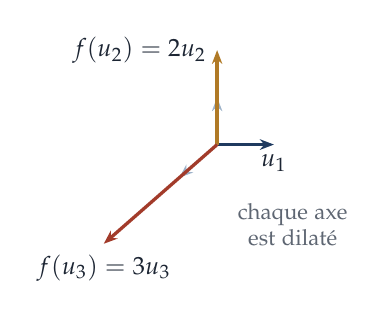
\begin{tikzpicture}[scale=0.6,>={Stealth[length=5pt]}]
  \draw[->,BleuClair,thick] (0,0)--(1.2,0) node[below,font=\small,Ink]{$u_1$};
  \draw[->,Bleu,very thick] (0,0)--(1.2,0);
  \draw[->,BleuClair,thick] (0,0)--(0,1);
  \draw[->,Ocre,very thick] (0,0)--(0,2) node[left,font=\small,Ink]{$f(u_2)=2u_2$};
  \draw[->,BleuClair,thick] (0,0)--(-0.8,-0.7);
  \draw[->,Brique,very thick] (0,0)--(-2.4,-2.1) node[below,font=\small,Ink]{$f(u_3)=3u_3$};
  \node[font=\footnotesize\color{Gris},align=center] at (1.6,-1.7) {chaque axe\\ est dilaté};
\end{tikzpicture}
\end{columns}
\pause
\vspace{-6pt}
\begin{RETENIR}
Quels vecteurs sont \textbf{simplement dilatés} ? Comment les \textbf{trouver} ? En a-t-on \textbf{assez pour une base} ?
\end{RETENIR}
\end{frame}

% =====================================================================
\partie{1.1}{Semblables, sommes directes, trace}{Qu'est-ce qui ne dépend pas de la base ? Comment découper un espace en morceaux ?}{\rmI}

\begin{frame}{Changement de base, matrices semblables}
\begin{PROP}[Changement de base \livre{prop.~1.1}]
$P$ matrice de passage de $\mathcal B$ à $\mathcal B'$ (colonnes : vecteurs de $\mathcal B'$ en coordonnées dans $\mathcal B$) :
\[\Mat_{\mathcal B'}(f)=P^{-1}\,\Mat_{\mathcal B}(f)\,P.\]
\end{PROP}
\begin{DEF}
$A$ et $B$ sont \emph{semblables} s'il existe $P$ inversible avec $B=P^{-1}AP$ : même endomorphisme, deux bases.
\end{DEF}
\pause
\begin{RETENIR}
\textbf{Invariants de similitude} : rang, déterminant, trace, polynôme caractéristique, valeurs propres.\\
Deux matrices qui diffèrent par un invariant ne sont \emph{pas} semblables. (La réciproque est fausse.)
\end{RETENIR}
\end{frame}

\begin{frame}{Somme de plusieurs sous-espaces, somme directe}
\begin{columns}[T]
\column{0.58\textwidth}
\begin{DEF}
$F_1+\dots+F_p=\{x_1+\dots+x_p,\ x_i\in F_i\}$.\\
Somme \emph{directe} $F_1\oplus\dots\oplus F_p$ : décomposition \emph{unique}.
\end{DEF}
\begin{PROP}[Caractérisation \livre{prop.~1.4}]
Directe $\iff$ \big($x_1+\dots+x_p=0$, $x_i\in F_i\Rightarrow$ tous nuls\big).\\
Pour deux : $F\cap G=\{0\}$.
\end{PROP}
\pause
\begin{PROP}[Base adaptée \livre{th.~1.5}]
Somme directe : bases concaténées $=$ base ;\ $\dim\bigoplus F_i=\sum\dim F_i$.
\end{PROP}
\column{0.38\textwidth}
\begin{PIEGE}[Trois droites du plan]
\centering
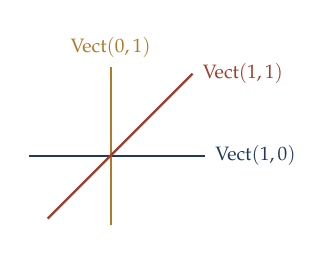
\begin{tikzpicture}[scale=0.8]
  \draw[Bleu,thick] (-1.3,0)--(1.5,0) node[right,font=\scriptsize]{$\vect(1,0)$};
  \draw[Ocre,thick] (0,-1.1)--(0,1.4) node[above,font=\scriptsize]{$\vect(0,1)$};
  \draw[Brique,thick] (-1,-1)--(1.3,1.3) node[right,font=\scriptsize]{$\vect(1,1)$};
\end{tikzpicture}\\[2pt]
\raggedright Intersections deux à deux nulles, mais $(1,0)+(0,1)-(1,1)=0$ : \textbf{pas directe}.
\end{PIEGE}
\end{columns}
{\small En dimension finie : $E=F\oplus G\iff F\cap G=\{0\}$ \ et \ $\dim F+\dim G=\dim E$.}
\end{frame}

% ---------------------------------------------------------------- EXERCICE 1
\begin{frame}{\badgeexo{1}Un plan et une droite}
\begin{ENONCE}[4 min]
Dans $\R^3$, soit $F$ le plan d'équation $x-y+2z=0$.
\begin{enumerate}
\item Montrer que $G=\vect\big((1,1,1)\big)$ est un supplémentaire de $F$, et décomposer $v=(x,y,z)$ selon $\R^3=F\oplus G$.
\item $H=\vect\big((1,1,0)\big)$ est-il un supplémentaire de $F$ ?
\end{enumerate}
\objectif{la caractérisation par l'intersection et les dimensions.}
\end{ENONCE}
\pause
\begin{INDICE}
Écrire $v=w+m(1,1,1)$ avec $w\in F$, et reporter dans l'équation de $F$.
\end{INDICE}
\end{frame}

\begin{frame}{\badgecor{1}Un plan et une droite}
\begin{columns}[T]
\column{0.4\textwidth}
\begin{RAIS}
Une droite $\vect(u)$ est un supplémentaire d'un plan $F$ de $\R^3$ exactement quand $u\notin F$ : intersection nulle, et $2+1=3$.
\end{RAIS}
\begin{OUTIL}
$E=F\oplus G\iff F\cap G=\{0\}$ et $\dim F+\dim G=\dim E$.
\end{OUTIL}
\column{0.57\textwidth}
\etape{1.} $(1,1,1)$ : $1-1+2=2\neq0$, donc $(1,1,1)\notin F$ : $F\cap G=\{0\}$, et $2+1=3$ : $\R^3=F\oplus G$.\\[3pt]
\pause
Si $v=w+m(1,1,1)$, $w\in F$ : $(x-m)-(y-m)+2(z-m)=0$, donc
\[m=\frac{x-y+2z}2,\qquad v=\underbrace{v-m(1,1,1)}_{\in F}+\underbrace{m(1,1,1)}_{\in G}.\]
\pause
\etape{2.} $1-1+0=0$ : $(1,1,0)\in F$, donc $H\subset F$ : \textbf{non}.
\end{columns}
\end{frame}

\begin{frame}{La trace}
\begin{columns}[T]
\column{0.55\textwidth}
\begin{DEF}
$\tr(A)=\sum_{i=1}^na_{i,i}$ : somme des coefficients diagonaux.
\end{DEF}
\begin{PROP}[\livre{prop.~1.7}]
\begin{itemize}
\item $\tr$ est linéaire ;
\item $\tr(AB)=\tr(BA)$ ;
\item $\tr(P^{-1}AP)=\tr(A)$ : on définit $\tr(f)$.
\end{itemize}
\end{PROP}
\column{0.41\textwidth}
\pause
\textbf{Preuve :}
\[\tr(AB)=\sum_{i,k}a_{i,k}b_{k,i}=\tr(BA).\]
Puis $\tr\big((P^{-1}A)P\big)=\tr\big(P(P^{-1}A)\big)=\tr A$.
\end{columns}
\pause
\begin{columns}[T]
\column{0.48\textwidth}
\begin{EX}[Projecteur]
Base adaptée : $\mathrm{diag}(I_r,0)$, donc $\tr(p)=r=\rg(p)$.
\end{EX}
\column{0.48\textwidth}
\begin{PIEGE}
$\tr(AB)\neq\tr A\,\tr B$ ; \ $\tr(ABC)\neq\tr(BAC)$ en général.
\end{PIEGE}
\end{columns}
\end{frame}

% ---------------------------------------------------------------- EXERCICE 2
\begin{frame}{\badgeexo{2}Semblables ou non ?}
\begin{ENONCE}[5 min]
Les matrices suivantes sont-elles semblables ? Justifier en une ligne.
\[\text{(a)}\ \begin{pmatrix}1&2\\0&3\end{pmatrix}\ \text{et}\ \begin{pmatrix}2&0\\1&2\end{pmatrix}\qquad
\text{(b)}\ I_2\ \text{et}\ \begin{pmatrix}1&1\\0&1\end{pmatrix}\qquad
\text{(c)}\ \begin{pmatrix}1&0\\0&0\end{pmatrix}\ \text{et}\ \begin{pmatrix}0&0\\0&0\end{pmatrix}\]
\objectif{utiliser les invariants, et voir leurs limites.}
\end{ENONCE}
\pause
\begin{INDICE}
Comparer trace, déterminant, rang. En (b), quelles sont les matrices semblables à $I_2$ ?
\end{INDICE}
\end{frame}

\begin{frame}{\badgecor{2}Semblables ou non ?}
\begin{columns}[T]
\column{0.4\textwidth}
\begin{RAIS}
Un invariant différent suffit pour dire \emph{non}. Mais des invariants égaux ne suffisent pas pour dire \emph{oui}.
\end{RAIS}
\begin{OUTIL}
Rang, trace, déterminant invariants par similitude.
\end{OUTIL}
\column{0.57\textwidth}
\etape{(a)} Même trace $4$, mais déterminants $3$ et $4$ : \textbf{non}.\\[4pt]
\pause
\etape{(b)} Même trace $2$, même déterminant $1$, même rang\dots\ mais $P^{-1}I_2P=I_2$ pour toute $P$ : la seule matrice semblable à $I_2$ est $I_2$. \textbf{Non}.\\[4pt]
\pause
\etape{(c)} Rangs $1$ et $0$ : \textbf{non}.
\end{columns}
\begin{ASTU}
(b) prépare le §1.5 : $\begin{pmatrix}1&1\\0&1\end{pmatrix}$ ne sera pas diagonalisable.
\end{ASTU}
\end{frame}

\begin{frame}{Hyperplans}
\begin{DEF}
Hyperplan de $E$ ($\dim E=n$) : sous-espace qui admet une droite comme supplémentaire ; dimension $n-1$.
\end{DEF}
\begin{PROP}[\livre{prop.~1.10}]
\begin{itemize}
\item Hyperplans $=$ noyaux des formes linéaires non nulles : une équation $a_1x_1+\dots+a_nx_n=0$.
\item $H=\Ker\varphi$, $u\notin H$ $\Rightarrow$ $E=H\oplus\vect(u)$ \quad (exercice~1).
\item $p$ hyperplans : intersection de dimension $\geq n-p$ ; un sous-espace de dimension $n-p$ est défini par $p$ équations.
\end{itemize}
\end{PROP}
\begin{EX}[Lecture géométrique]
Dans $\R^3$ : un plan vectoriel $=$ une équation ; une droite $=$ deux équations (deux plans qui se coupent).
\end{EX}
\end{frame}

% =====================================================================
\partie{1.2}{Sous-espaces stables}{Comment lire sur une matrice qu'un sous-espace est « respecté » par $f$ ?}{\rmI}

\begin{frame}{Sous-espace stable, endomorphisme induit}
\begin{DEF}
$F$ est \emph{stable} par $f$ si $f(F)\subset F$. L'endomorphisme induit $f_F:F\to F$, $x\mapsto f(x)$.
\end{DEF}
\begin{PROP}[\livre{prop.~1.12}]
\begin{itemize}
\item $F=\vect(e_1,\dots,e_p)$ stable $\iff f(e_j)\in F$ pour tout $j$ : on vérifie sur une base.
\item $\Ker f$ et $\Im f$ sont stables par $f$ ; si $f\circ g=g\circ f$, $\Ker g$ et $\Im g$ sont stables par $f$.
\end{itemize}
\end{PROP}
\pause
\textbf{Preuve du second point :} $g(x)=0\Rightarrow g\big(f(x)\big)=f\big(g(x)\big)=0$ ; \ $f\big(g(x)\big)=g\big(f(x)\big)\in\Im g$.
\end{frame}

\begin{frame}{Traduction matricielle : des blocs}
\begin{columns}[c]
\column{0.58\textwidth}
\begin{PROP}[Théorème \livre{th.~1.13}]
Base adaptée à $F$ ($p$ premiers vecteurs dans $F$) :
\[F\text{ stable}\iff\Mat(f)=\begin{pmatrix}A&B\\0&C\end{pmatrix}.\]
$E=F\oplus G$, les deux stables $\iff\begin{pmatrix}A&0\\0&C\end{pmatrix}$.\\
Alors $\det f=\det A\det C$, \ $\tr f=\tr A+\tr C$.
\end{PROP}
\column{0.38\textwidth}
\centering
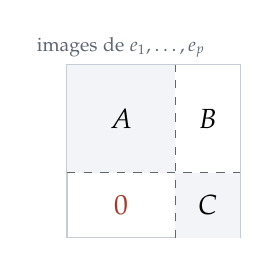
\begin{tikzpicture}[scale=0.55]
  \draw[Filet] (0,0) rectangle (4,4);
  \fill[Fond] (0,1.5) rectangle (2.5,4); \node at (1.25,2.75) {$A$};
  \node at (3.25,2.75) {$B$};
  \node[Brique] at (1.25,0.75) {$0$};
  \fill[Fond] (2.5,0) rectangle (4,1.5); \node at (3.25,0.75) {$C$};
  \draw[Gris,dashed] (2.5,0)--(2.5,4); \draw[Gris,dashed] (0,1.5)--(4,1.5);
  \node[font=\scriptsize,Gris] at (1.25,4.4) {images de $e_1,\dots,e_p$};
\end{tikzpicture}\\[2pt]
{\footnotesize\color{Gris}le $0$ dit : les $f(e_j)$, $j\leq p$, restent dans $F$}
\end{columns}
\pause
\begin{columns}[T]
\column{0.58\textwidth}
\begin{FORM}[Projecteurs, symétries]
$p^2=p$ : $\mathrm{diag}(I_r,0)$ dans $\Im p\oplus\Ker p$.\\
$s^2=\Id$ : $\mathrm{diag}(I_r,-I_{n-r})$ dans $\Ker(s-\Id)\oplus\Ker(s+\Id)$.
\end{FORM}
\column{0.38\textwidth}
\begin{PROP}[Droite stable \livre{prop.~1.14}]
$\vect(u)$ stable $\iff f(u)=\lambda u$.
\end{PROP}
\end{columns}
\end{frame}

% ---------------------------------------------------------------- EXERCICE 3
\begin{frame}{\badgeexo{3}Chercher des droites stables}
\begin{ENONCE}[6 min]
Soit $f$ l'endomorphisme de $\R^3$ de matrice $A=\begin{pmatrix}1&2&0\\2&1&0\\0&0&-1\end{pmatrix}$.
\begin{enumerate}
\item Montrer que le plan $F$ : $z=0$ et la droite $\vect(e_3)$ sont stables par $f$. Que dit la forme de $A$ ?
\item Montrer que les droites engendrées par $(1,1,0)$ et $(1,-1,0)$ sont stables.
\item En déduire une base dans laquelle la matrice de $f$ est diagonale.
\end{enumerate}
\objectif{passer des sous-espaces stables aux vecteurs propres.}
\end{ENONCE}
\end{frame}

\begin{frame}{\badgecor{3}Chercher des droites stables}
\begin{columns}[T]
\column{0.4\textwidth}
\begin{RAIS}
Les blocs se lisent sur $A$ ; une droite est stable quand son vecteur directeur est dilaté. Trois droites stables
supplémentaires : matrice diagonale.
\end{RAIS}
\begin{OUTIL}
Théorème~1.13 ; proposition~1.14.
\end{OUTIL}
\column{0.57\textwidth}
\etape{1.} $f(x,y,0)=(x+2y,2x+y,0)\in F$ ; $f(e_3)=-e_3$. $A$ est diagonale par blocs : $\begin{pmatrix}A_1&0\\0&-1\end{pmatrix}$.\\[3pt]
\pause
\etape{2.} $A(1,1,0)^T=(3,3,0)^T$ : dilatation de rapport $3$. $A(1,-1,0)^T=(-1,1,0)^T$ : rapport $-1$.\\[3pt]
\pause
\etape{3.} $\mathcal B'=\big((1,1,0),(1,-1,0),e_3\big)$ est une base (déterminant non nul), et
\[\Mat_{\mathcal B'}(f)=\mathrm{diag}(3,-1,-1).\]
\end{columns}
\begin{ASTU}
Ces vecteurs, simplement dilatés, sont les \emph{vecteurs propres} : c'est la notion suivante.
\end{ASTU}
\end{frame}

% =====================================================================
\partie{1.3}{Éléments propres}{Quels vecteurs sont simplement dilatés par $f$ ?}{\rmI}

\begin{frame}{Valeurs propres, vecteurs propres, sous-espaces propres}
\begin{DEF}[Définition \livre{déf.~1.15}]
\begin{itemize}
\item $\lambda$ est \emph{valeur propre} de $f$ s'il existe $x\neq0$ tel que $f(x)=\lambda x$ ; $x$ est un \emph{vecteur propre} (\alert{non nul}).
\item Sous-espace propre : $E_\lambda(f)=\Ker(f-\lambda\Id_E)$. \quad Spectre (dimension finie) : $\Sp(f)$.
\end{itemize}
\end{DEF}
\pause
\begin{columns}[T]
\column{0.48\textwidth}
\begin{RETENIR}
$E_\lambda$ est un sous-espace, stable par $f$, $\neq\{0\}$ exactement si $\lambda\in\Sp(f)$.\\
$0\in\Sp(f)\iff f$ non injective ; $E_0=\Ker f$.
\end{RETENIR}
\column{0.48\textwidth}
\begin{EX}[Dimension infinie]
$D:y\mapsto y'$ sur $\mathcal C^\infty$ : $y'=\lambda y$, donc $E_\lambda=\vect(e^{\lambda t})$ (chapitre 1).\\
$P\mapsto XP'$ : $X^k$, valeur propre $k$.
\end{EX}
\end{columns}
\end{frame}

\begin{frame}{Des vecteurs propres de valeurs distinctes sont libres}
\begin{PROP}[Théorème \livre{th.~1.18}]
Pour des valeurs propres \emph{distinctes} $\lambda_1,\dots,\lambda_p$, la somme $E_{\lambda_1}+\dots+E_{\lambda_p}$ est directe.
Une famille de vecteurs propres de valeurs propres distinctes est libre. En dimension $n$ : au plus $n$ valeurs propres.
\end{PROP}
\pause
\textbf{Idée de la preuve} (récurrence) : si $x_1+\dots+x_p=0$, on applique $f$ et on retranche $\lambda_p\times$ la relation :
\[(\lambda_1-\lambda_p)x_1+\dots+(\lambda_{p-1}-\lambda_p)x_{p-1}=0\ \Rightarrow\ x_1=\dots=x_{p-1}=0\ \Rightarrow\ x_p=0.\]
\pause
\begin{METH}{Déterminer $E_\lambda(A)$ \livre{méth.~1.1}}
Résoudre $(A-\lambda I_n)X=0$ ;\quad $\dim E_\lambda=n-\rg(A-\lambda I_n)$ \ (théorème du rang) : \textbf{le rang d'abord}.
\end{METH}
\end{frame}

% ---------------------------------------------------------------- EXERCICE 4
\begin{frame}{\badgeexo{4}Éléments propres sans matrice}
\begin{ENONCE}[6 min]
\begin{enumerate}
\item Sur $\R_n[X]$, soit $s(P)=P(-X)$. Déterminer ses valeurs propres et ses sous-espaces propres.
\item Sur $\R_2[X]$, soit $D(P)=P'$. Montrer que $0$ est la seule valeur propre de $D$, et déterminer $E_0(D)$.
Existe-t-il une base de $\R_2[X]$ formée de vecteurs propres de $D$ ?
\end{enumerate}
\objectif{écrire directement $f(P)=\lambda P$.}
\end{ENONCE}
\pause
\begin{INDICE}
(1) $s\circ s=\Id$. \quad (2) Si $P'=\lambda P$ avec $\lambda\neq0$, comparer les degrés.
\end{INDICE}
\end{frame}

\begin{frame}{\badgecor{4}Éléments propres sans matrice}
\begin{columns}[T]
\column{0.4\textwidth}
\begin{RAIS}
On écrit l'équation aux éléments propres dans l'espace lui-même ; un argument de degré ou une relation $s^2=\Id$ suffit.
\end{RAIS}
\begin{OUTIL}
Définition ; $E_\lambda=\Ker(f-\lambda\Id)$.
\end{OUTIL}
\column{0.57\textwidth}
\etape{1.} $s\circ s=\Id$ : si $s(P)=\lambda P$, $P\neq0$, alors $P=\lambda^2P$, $\lambda=\pm1$.
$E_1$ : polynômes pairs ; $E_{-1}$ : polynômes impairs. (Et $\R_n[X]=E_1\oplus E_{-1}$.)\\[3pt]
\pause
\etape{2.} Si $P'=\lambda P$, $\lambda\neq0$, $P\neq0$ : $\deg P'<\deg P=\deg(\lambda P)$, impossible. $\lambda=0$ : $P'=0$,
$E_0(D)=\R_0[X]$ (constantes), de dimension $1$.\\[3pt]
\pause
Les vecteurs propres sont tous constants : \textbf{pas de base} de vecteurs propres ($\dim\R_2[X]=3$).
\end{columns}
\begin{ASTU}
$D$ sera notre premier exemple d'endomorphisme \emph{non diagonalisable}.
\end{ASTU}
\end{frame}

% =====================================================================
\partie{1.4}{Polynôme caractéristique}{Comment trouver les valeurs propres d'une matrice ?}{\rmI}

\begin{frame}{Le polynôme caractéristique}
\[\lambda\in\Sp(A)\iff A-\lambda I_n\text{ non inversible}\iff\det(\lambda I_n-A)=0.\]
\pause
\begin{PROP}[\livre{prop.~1.21, th.~1.22}]
$\chi_A(x)=\det(xI_n-A)$ est un polynôme \textbf{unitaire} de degré $n$ :
\[\chi_A(x)=x^n-\tr(A)\,x^{n-1}+\dots+(-1)^n\det A\qquad(n=2 :\ x^2-\tr(A)\,x+\det A).\]
$\Sp(A)$ = racines de $\chi_A$ \emph{dans $\K$} ; \ semblables $\Rightarrow$ même $\chi$ (on définit $\chi_f$) ;\\
triangulaire : $\chi_A=\prod(x-a_{i,i})$, valeurs propres sur la diagonale.
\end{PROP}
\pause
\begin{PIEGE}
$\det(A-xI_n)=(-1)^n\chi_A(x)$ : mêmes racines, mais $\chi_A$ est \emph{unitaire}.
\end{PIEGE}
\end{frame}

\begin{frame}{Multiplicité et dimension}
\begin{PROP}[Théorème \livre{th.~1.24}]
$m(\lambda)$ : multiplicité de $\lambda$ comme racine de $\chi_f$.\qquad $1\leq\dim E_\lambda(f)\leq m(\lambda)$.
\end{PROP}
\pause
\begin{columns}[c]
\column{0.55\textwidth}
\textbf{Preuve :} $E_\lambda$ est stable ; base adaptée :
\[\Mat(f)=\begin{pmatrix}\lambda I_d&B\\0&C\end{pmatrix},\quad\chi_f=(x-\lambda)^d\,\chi_C.\]
Donc $(x-\lambda)^d$ divise $\chi_f$ : $d\leq m(\lambda)$.
\column{0.4\textwidth}
\begin{RETENIR}
Valeur propre \textbf{simple} $\Rightarrow\dim E_\lambda=1$.\\
Valeur multiple : \textbf{tout est possible} entre $1$ et $m(\lambda)$.
\end{RETENIR}
\end{columns}
\pause
\begin{METH}{Calculer $\chi_A$ ($n=3$) \livre{méth.~1.2}}
Chercher une structure (somme des lignes constante, colonne qui fait apparaître un facteur, zéros) ; \textbf{factoriser au fur et à mesure}.
Contrôles : somme des racines $=\tr A$, produit $=\det A$.
\end{METH}
\end{frame}

% ---------------------------------------------------------------- EXERCICE 5
\begin{frame}{\badgeexo{5}Valeurs propres et dimensions}
\begin{ENONCE}[7 min]
Soit $K=\begin{pmatrix}1&1&0\\1&1&0\\1&-1&2\end{pmatrix}$.
\begin{enumerate}
\item Calculer $\chi_K$ sous forme factorisée, et contrôler avec la trace et le déterminant.
\item Pour chaque valeur propre, donner la multiplicité, puis $\dim E_\lambda$ (par un rang).
\item Déterminer une base de chaque sous-espace propre.
\end{enumerate}
\objectif{le calcul de $\chi$ par un développement bien choisi, puis le rang.}
\end{ENONCE}
\pause
\begin{INDICE}
Dans $xI_3-K$, la troisième colonne n'a qu'un coefficient non nul.
\end{INDICE}
\end{frame}

\begin{frame}{\badgecor{5}Valeurs propres et dimensions}
\begin{columns}[T]
\column{0.38\textwidth}
\begin{RAIS}
Développer selon la colonne à deux zéros : le facteur $(x-2)$ sort. Puis $\dim E_\lambda=3-\rg(K-\lambda I_3)$.
\end{RAIS}
\begin{OUTIL}
Méthodes~1.1 et~1.2 ; théorème~1.24.
\end{OUTIL}
\column{0.59\textwidth}
\etape{1.} $\chi_K=(x-2)\dt{x-1&-1\\-1&x-1}=(x-2)\big((x-1)^2-1\big)=x(x-2)^2.$\\
Contrôle : $0+2+2=4=\tr K$ ; \ $\det K=0$.\\[3pt]
\pause
\etape{2.} $0$ simple : $\dim E_0=1$. \ $2$ double :
$K-2I_3=\begin{pmatrix}-1&1&0\\1&-1&0\\1&-1&0\end{pmatrix}$, rang $1$, $\dim E_2=2=m(2)$.\\[3pt]
\pause
\etape{3.} $E_2$ : $x=y$, base $(1,1,0)$, $(0,0,1)$. \ $E_0$ : $x+y=0$, $x-y+2z=0$ : $(1,-1,-1)$.
\end{columns}
\begin{ASTU}
$\dim E_0+\dim E_2=3$ : base de vecteurs propres (critère du §1.5).
\end{ASTU}
\end{frame}

% =====================================================================
\partie{1.5}{Diagonalisation}{Quand a-t-on assez de vecteurs propres pour former une base ?}{\rmI}

\begin{frame}{Diagonalisable : définition et critères}
\begin{DEF}
$f$ diagonalisable : il existe une base de \emph{vecteurs propres}.\
$A$ diagonalisable : $A=PDP^{-1}$, colonnes de $P$ = vecteurs propres, $D$ = valeurs propres \emph{dans le même ordre}.
\end{DEF}
\pause
\begin{PROP}[Critères \livre{th.~1.27}]
$f$ diagonalisable $\iff E=\bigoplus_\lambda E_\lambda\iff\sum_\lambda\dim E_\lambda=n$\\
\hspace*{2.95cm}$\iff\chi_f$ scindé \textbf{et} $\dim E_\lambda=m(\lambda)$ pour toute valeur propre.
\end{PROP}
\pause
\begin{columns}[T]
\column{0.5\textwidth}
\begin{RETENIR}
$n$ valeurs propres \textbf{distinctes} $\Rightarrow$ diagonalisable \livre{cor.~1.28}. Réciproque fausse ($I_n$).
\end{RETENIR}
\column{0.46\textwidth}
\begin{ASTU}[Réflexe]
Diagonalisable avec une seule valeur propre $\lambda$ $\Rightarrow A=P(\lambda I_n)P^{-1}=\lambda I_n$.
\end{ASTU}
\end{columns}
\end{frame}

\begin{frame}{La méthode, sur un exemple}
\begin{METH}{Diagonaliser \livre{méth.~1.3}}
(1) $\chi_A$ factorisé \ (2) valeurs simples : oui ; multiples : $\dim E_\lambda$ vs $m(\lambda)$ \ (3) bases des $E_\lambda$ en colonnes : $P$ \ (4) contrôle $AP=PD$.
\end{METH}
\pause
$A=\begin{pmatrix}5&1&-1\\2&4&-2\\1&-1&3\end{pmatrix}$. Dans $xI_3-A$, $C_2\leftarrow C_2+C_3$ donne $(0,x-2,x-2)$ :
\ $\chi_A=(x-2)\big((x-5)^2-1\big)=(x-2)(x-4)(x-6)$.\\[4pt]
\pause
Trois valeurs distinctes : diagonalisable. \ $E_2=\vect(0,1,1)$, $E_4=\vect(1,0,1)$, $E_6=\vect(1,1,0)$ :
\[P=\begin{pmatrix}0&1&1\\1&0&1\\1&1&0\end{pmatrix},\qquad D=\mathrm{diag}(2,4,6).\]
\end{frame}

% ---------------------------------------------------------------- EXERCICE 6
\begin{frame}{\badgeexo{6}Diagonalisable ou non ?}
\begin{ENONCE}[5 min]
Sans calcul long, dire si chaque matrice est diagonalisable dans $\mathcal M_n(\R)$, puis dans $\mathcal M_n(\C)$.
\[\text{(a)}\begin{pmatrix}1&1\\0&2\end{pmatrix}\quad\text{(b)}\begin{pmatrix}3&1\\0&3\end{pmatrix}\quad\text{(c)}\begin{pmatrix}0&-1\\1&0\end{pmatrix}\quad
\text{(d)}\begin{pmatrix}1&1\\1&1\end{pmatrix}\quad\text{(e)}\begin{pmatrix}2&0&0\\0&2&0\\0&0&5\end{pmatrix}\]
\objectif{choisir le bon critère en quelques secondes.}
\end{ENONCE}
\end{frame}

\begin{frame}{\badgecor{6}Diagonalisable ou non ?}
\begin{columns}[T]
\column{0.38\textwidth}
\begin{RAIS}
Avant tout calcul : triangulaire ? valeurs distinctes ? une seule valeur propre ? $\chi$ scindé ? rang $1$ ?
\end{RAIS}
\begin{OUTIL}
Corollaire~1.28 ; réflexe « une seule valeur propre » ; $\chi$ scindé.
\end{OUTIL}
\column{0.59\textwidth}
\etape{(a)} Triangulaire, valeurs $1\neq2$ : \textbf{oui} (sur $\R$ et $\C$).\\[2pt]
\etape{(b)} Seule valeur propre $3$, et $\neq3I_2$ : \textbf{non}, ni sur $\R$ ni sur $\C$.\\[2pt]
\pause
\etape{(c)} $\chi=x^2+1$ : \textbf{non} sur $\R$ ; $\pm i$ distinctes : \textbf{oui} sur $\C$.\\[2pt]
\etape{(d)} Rang $1$ : $\dim E_0=1$ ; $\tr=2$ : valeur propre $2$. Valeurs $0\neq2$ : \textbf{oui}.\\[2pt]
\etape{(e)} Déjà diagonale : \textbf{oui}.
\end{columns}
\begin{PIEGE}
(e) a une valeur propre double et \emph{est} diagonalisable : une valeur multiple n'empêche rien, il faut comparer $\dim E_\lambda$ et $m(\lambda)$.
\end{PIEGE}
\end{frame}

% ---------------------------------------------------------------- EXERCICE 7
\begin{frame}{\badgeexo{7}Diagonaliser, avec une valeur propre double}
\begin{ENONCE}[8 min]
Diagonaliser $A=\begin{pmatrix}2&0&1\\0&1&0\\1&0&2\end{pmatrix}$ : donner $P$ inversible et $D$ diagonale telles que $A=PDP^{-1}$, puis
vérifier $AP=PD$ sur une colonne.
\objectif{la méthode complète, avec comparaison dimension--multiplicité.}
\end{ENONCE}
\pause
\begin{INDICE}
Développer $\chi_A$ selon la deuxième ligne.
\end{INDICE}
\end{frame}

\begin{frame}{\badgecor{7}Diagonaliser, avec une valeur propre double}
\begin{columns}[T]
\column{0.38\textwidth}
\begin{RAIS}
Une ligne presque nulle donne un facteur ; pour la valeur double, le rang de $A-\lambda I_3$ décide.
\end{RAIS}
\begin{OUTIL}
Méthode~1.3 ; critère $\dim E_\lambda=m(\lambda)$.
\end{OUTIL}
\column{0.59\textwidth}
\etape{1.} $\chi_A=(x-1)\big((x-2)^2-1\big)=(x-1)^2(x-3)$.\\[2pt]
\pause
\etape{2.} $A-I_3=\begin{pmatrix}1&0&1\\0&0&0\\1&0&1\end{pmatrix}$, rang $1$ : $\dim E_1=2=m(1)$ : diagonalisable.\\[2pt]
\pause
\etape{3.} $E_1$ : $x+z=0$, base $(0,1,0)$, $(-1,0,1)$ ; \ $E_3=\vect(1,0,1)$.
\[P=\begin{pmatrix}0&-1&1\\1&0&0\\0&1&1\end{pmatrix},\quad D=\mathrm{diag}(1,1,3).\]
\etape{4.} $A(1,0,1)^T=(3,0,3)^T$ : troisième colonne de $PD$.
\end{columns}
\end{frame}

% =====================================================================
\partie{1.6}{Applications}{Que gagne-t-on à diagonaliser ?}{\rmI}

\begin{frame}{Puissances, suites couplées}
\begin{PROP}[\livre{prop.~1.33}]
$A=PDP^{-1}\Rightarrow A^k=PD^kP^{-1}$, \ $D^k=\mathrm{diag}(\lambda_1^k,\dots,\lambda_n^k)$ ; \ $k\in\Z$ si $A$ est inversible.
\end{PROP}
\pause
\begin{METH}{Suites couplées \livre{méth.~1.4}}
$X_{k+1}=AX_k\Rightarrow X_k=A^kX_0$. Dans la base propre, $Y_k=P^{-1}X_k$ vérifie $Y_{k+1}=DY_k$ : des suites \textbf{géométriques}.
\end{METH}
\pause
\begin{EX}
$u_{k+1}=u_k+2v_k$, $v_{k+1}=2u_k+v_k$. Valeurs propres $3$ et $-1$, vecteurs $(1,1)$, $(1,-1)$. Coordonnées propres : $s_k=u_k+v_k$, $d_k=u_k-v_k$,
avec $s_{k+1}=3s_k$, $d_{k+1}=-d_k$. \ Donc $u_k=\frac{3^ks_0+(-1)^kd_0}2$.
\end{EX}
\end{frame}

\begin{frame}{Équations matricielles}
\begin{PROP}[\livre{prop.~1.35}]
$D$ diagonale à coefficients \textbf{distincts} : $MD=DM\iff M$ diagonale \quad (coefficient $(i,j)$ : $m_{i,j}(d_j-d_i)$).
\end{PROP}
\pause
\begin{METH}{Passer dans la base propre}
$A=PDP^{-1}$ : poser $N=P^{-1}MP$ ; l'équation sur $M$ devient la même sur $N$, avec $D$.
\end{METH}
\begin{EX}[$M^2=A$, $A$ de valeurs propres $1,4,9$]
$M$ commute avec $M^2=A$, donc $N$ commute avec $D$ : $N$ diagonale, $N^2=D$ : $N=\mathrm{diag}(\pm1,\pm2,\pm3)$, \textbf{8 solutions}.
\end{EX}
\begin{HPBOX}
Polynômes d'endomorphismes ; systèmes $X'=AX$ (ils se traiteraient comme les suites, avec $Y=P^{-1}X$).
\end{HPBOX}
\end{frame}

% ---------------------------------------------------------------- EXERCICE 8
\begin{frame}{\badgeexo{8}La suite de Fibonacci}
\begin{ENONCE}[8 min]
$F_0=0$, $F_1=1$, $F_{k+2}=F_{k+1}+F_k$. On pose $X_k=\begin{pmatrix}F_k\\F_{k+1}\end{pmatrix}$.
\begin{enumerate}
\item Trouver $A$ telle que $X_{k+1}=AX_k$. Montrer que $A$ est diagonalisable dans $\mathcal M_2(\R)$.
\item En déduire $F_k=\dfrac{\varphi^k-\psi^k}{\sqrt5}$, où $\varphi=\frac{1+\sqrt5}2$ et $\psi=\frac{1-\sqrt5}2$.
\item Limite de $\dfrac{F_{k+1}}{F_k}$ ?
\end{enumerate}
\objectif{exploiter $A^k=PD^kP^{-1}$ sans calculer $P^{-1}$ en entier.}
\end{ENONCE}
\pause
\begin{INDICE}
$\chi_A=x^2-x-1$. Toute coordonnée de $X_k$ est combinaison fixe de $\varphi^k$ et $\psi^k$ : utiliser $F_0$ et $F_1$.
\end{INDICE}
\end{frame}

\begin{frame}{\badgecor{8}La suite de Fibonacci}
\begin{columns}[T]
\column{0.4\textwidth}
\begin{RAIS}
Une récurrence linéaire est un $X_{k+1}=AX_k$. Diagonaliser $A$ montre que $F_k=\alpha\varphi^k+\beta\psi^k$ ; deux conditions
fixent $\alpha$, $\beta$.
\end{RAIS}
\begin{OUTIL}
$\chi=x^2-\tr\,x+\det$ ; corollaire~1.28 ; $A^k=PD^kP^{-1}$.
\end{OUTIL}
\column{0.57\textwidth}
\etape{1.} $A=\begin{pmatrix}0&1\\1&1\end{pmatrix}$, $\chi_A=x^2-x-1$, racines $\varphi\neq\psi$ réelles : diagonalisable.\\[3pt]
\pause
\etape{2.} $X_k=PD^kP^{-1}X_0$ : $F_k=\alpha\varphi^k+\beta\psi^k$. Avec $F_0=0$ : $\beta=-\alpha$ ; $F_1=1$ : $\alpha(\varphi-\psi)=1$, $\alpha=\frac1{\sqrt5}$.\\[3pt]
\pause
\etape{3.} $|\psi|<1<\varphi$ : $F_k\sim\frac{\varphi^k}{\sqrt5}$, donc $\dfrac{F_{k+1}}{F_k}\to\varphi$ (nombre d'or).
\end{columns}
\begin{ASTU}
La plus grande valeur propre (en module) dicte le comportement à l'infini.
\end{ASTU}
\end{frame}

% =====================================================================
\partie{1.7}{Trigonalisation}{Et quand ce n'est pas diagonalisable ?}{\rmI}

\begin{frame}{Trigonaliser ; trace et déterminant}
\begin{PROP}[\livre{th.~1.37, prop.~1.38}]
Trigonalisable (semblable à une triangulaire) $\iff\chi$ scindé \ (\emph{admis}). Toute matrice de $\Mn{\C}$ est trigonalisable.\\
Si $\chi_A=\prod(x-\lambda_i)$ (avec multiplicités) :\qquad $\tr A=\sum\lambda_i$,\qquad $\det A=\prod\lambda_i$.
\end{PROP}
{\footnotesize\color{Gris}Aucune technique générale de trigonalisation n'est au programme : les exercices la guident (TD, exercice~26).}
\pause
\begin{columns}[T]
\column{0.5\textwidth}
\begin{ASTU}
$\tr$ et $\det$ : somme et produit des valeurs propres \textbf{sans calcul}.\\
$\rg A=1$ : $0$ d'ordre $\geq n-1$, la dernière valeur propre est $\tr A$.
\end{ASTU}
\column{0.46\textwidth}
\begin{EX}[Nilpotente]
$A^p=0$, $AX=\lambda X$ : $\lambda^pX=0$, donc $\Sp_\C(A)=\{0\}$, $\chi_A=x^n$, $\tr A=0$. Diagonalisable $\iff A=0$.
\end{EX}
\end{columns}
\end{frame}

% ---------------------------------------------------------------- EXERCICE 9
\begin{frame}{\badgeexo{9}Valeurs propres en une ligne}
\begin{ENONCE}[4 min]
Sans calculer de polynôme caractéristique, donner les valeurs propres (avec multiplicités) et dire si la matrice est diagonalisable :
\[\text{(a)}\ \begin{pmatrix}1&1&1\\2&2&2\\3&3&3\end{pmatrix}\qquad\text{(b)}\ \begin{pmatrix}1&-1\\1&-1\end{pmatrix}\qquad
\text{(c)}\ B\in\mathcal M_2(\R)\text{ avec }\tr B=5,\ \det B=6.\]
\objectif{trace, déterminant, rang.}
\end{ENONCE}
\end{frame}

\begin{frame}{\badgecor{9}Valeurs propres en une ligne}
\begin{columns}[T]
\column{0.38\textwidth}
\begin{RAIS}
Le rang donne $\dim E_0$ ; la trace donne la somme des valeurs propres, le déterminant leur produit.
\end{RAIS}
\begin{OUTIL}
Proposition~1.38 ; théorème du rang.
\end{OUTIL}
\column{0.59\textwidth}
\etape{(a)} Rang $1$ : $\dim E_0=2$, donc $0$ d'ordre $\geq2$ ; la dernière vaut $\tr=6$. Valeurs $0,0,6$ ; $\dim E_0+\dim E_6=3$ :
\textbf{diagonalisable}.\\[3pt]
\pause
\etape{(b)} Rang $1$, $\tr=0$ : valeurs $0,0$ ; matrice non nulle : \textbf{non diagonalisable}.\\[3pt]
\pause
\etape{(c)} $\lambda_1+\lambda_2=5$, $\lambda_1\lambda_2=6$ : $2$ et $3$, distinctes : \textbf{diagonalisable}.
\end{columns}
\end{frame}

% =====================================================================
\partie{1.8}{Synthèse}{Devant une question d'algèbre linéaire, par quoi commencer ?}{\rmI}

\begin{frame}{Quelle méthode ?}
\small
\renewcommand{\arraystretch}{1.28}
\begin{tabular}{@{}p{4.6cm}p{9.2cm}@{}}
\toprule
\textbf{Question} & \textbf{Méthode}\\\midrule
$E=F\oplus G$ ? & intersection nulle et somme des dimensions\\
$F$ stable par $f$ ? & images d'une base de $F$ ; forme triangulaire par blocs\\
$\lambda$ valeur propre ? $\dim E_\lambda$ ? & $\rg(A-\lambda I_n)<n$ ; \ $\dim E_\lambda=n-\rg(A-\lambda I_n)$\\
valeurs propres & $\chi_A$ \textbf{factorisé} ; contrôle par $\tr$ et $\det$ ; ou rang, trace, relation ($A^2=I$, $A^p=0$\dots)\\
diagonalisable ? & distinctes ; sinon $\dim E_\lambda=m(\lambda)$ ; $\chi$ scindé ; « une seule valeur propre »\\
$A^k$, suites, équations & $A=PDP^{-1}$ ; travailler dans la base propre\\
endomorphisme de polynômes, de fonctions & écrire $f(x)=\lambda x$ directement (degré, $e^{\lambda t}$, parité)\\\bottomrule
\end{tabular}
\end{frame}

\begin{frame}{Pièges et essentiel}
\begin{columns}[T]
\column{0.48\textwidth}
\begin{PIEGE}[Pièges fréquents]
\begin{itemize}
\item Vecteur propre \emph{non nul}.
\item Somme directe de trois sous-espaces : les intersections deux à deux ne suffisent pas.
\item $\chi$ non scindé sur $\R$ (rotation).
\item Valeur double $\not\Rightarrow$ non diagonalisable.
\item Vecteurs propres en \emph{colonnes}, ordre de $D$.
\item $A=PDP^{-1}$, pas $P^{-1}DP$.
\end{itemize}
\end{PIEGE}
\column{0.48\textwidth}
\begin{RETENIR}
\begin{itemize}
\item Semblables : rang, $\tr$, $\det$, $\chi$ communs.
\item Stable $\iff$ blocs ; droite stable $\iff$ vecteur propre.
\item $\chi_A=\det(xI_n-A)$ ; $1\leq\dim E_\lambda\leq m(\lambda)$.
\item Diagonalisable $\iff\sum\dim E_\lambda=n$.
\item $A^k=PD^kP^{-1}$ ; $\tr=\sum\lambda_i$, $\det=\prod\lambda_i$.
\end{itemize}
\end{RETENIR}
\end{columns}
\end{frame}

\begin{frame}{Après la séance}
\begin{columns}[T]
\column{0.52\textwidth}
\begin{enumerate}
\item \textbf{Relire le livre} (chapitre~2) : démonstrations et exemples rédigés.
\item \textbf{Apprendre la fiche}.
\item \textbf{Cinq problèmes} de la sélection, dans l'ordre :
\begin{itemize}\small
\item diagonaliser pour calculer des puissances ;
\item un endomorphisme de $\R_n[X]$ ;
\item une matrice tridiagonale (lien avec les déterminants) ;
\item matrices qui commutent ;
\item l'endomorphisme $M\mapsto AM-MA$.
\end{itemize}
\item Puis le \textbf{TD complet} (29 exercices, quatre niveaux).
\end{enumerate}
\column{0.42\textwidth}
\begin{ASTU}[Pour chercher seul]
Lire l'en-tête du problème, chercher au brouillon, ne lire qu'\emph{une} indication en cas de blocage, la correction à la fin.
\end{ASTU}
\begin{ASTU}[Lien avec les déterminants]
Le polynôme caractéristique est un déterminant : toutes les techniques du chapitre \emph{Déterminants} servent ici.
\end{ASTU}
\end{columns}
\end{frame}

\end{document}
